\documentclass{beamer}

\mode<presentation> {
  \usetheme{CambridgeUS}
  %\setbeamertemplate{footline} % To remove the footer line in all slides uncomment this line
  %\setbeamertemplate{footline}[page number] % To replace the footer line in all slides with a simple slide count uncomment this line
  \setbeamertemplate{navigation symbols}{} % To remove the navigation symbols from the bottom of all slides uncomment this line
}

\usepackage{graphicx}
\usepackage{booktabs}
\usepackage{svg}

%----------------------------------------------------------------------------------------
%   TITLE PAGE
%----------------------------------------------------------------------------------------

\title[Project Object Recognition]{Physics Perception with Computer Vision}

\author{Louis THIRY, Marc SANSELME}
\institute[MVA]
{ENS-Cachan}
\date{\today}

\begin{document}

\begin{frame}
\titlepage
\end{frame}

%\begin{frame}
%\frametitle{Overview}
%\tableofcontents
%\end{frame}

%----------------------------------------------------------------------------------------
%   PRESENTATION SLIDES
%----------------------------------------------------------------------------------------

\section{Introduction}

\begin{frame}
\frametitle{Measure quantity with computer vision}
\begin{itemize}
  \item recording a video is easy
  \item thanks to computer vison, kinematic informations (velocity, acceleration...) can be measured
  \item thanks to mecanics, other quantities (mass, length...) can be deduced from these informations
\end{itemize}
$\rightarrow$ Proof of concept with a pendulum
\end{frame}

%\begin{frame}
%\frametitle{Simple pendulum}
%\begin{figure}
%  \captionsetup{labelformat=empty}
%  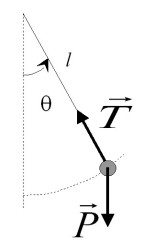
\includegraphics{pendule.jpg}
%  \caption{Simple pendulum}
%\end{figure}
%\begin{align*}
%  \ddot{\theta} + \frac{g}{l} \sin (\theta) = 0
%\end{align*}
%Simply depends on the length $\rightarrow$ deduce the length from the angle sequence
%\end{frame}

\begin{frame}
\frametitle{Methodology}
\begin{itemize}
  \item Computer Vision : Deduce the angle sequence from a video
  \item Learning : Deduce the length from the angle sequence
\end{itemize}
\end{frame}

\section{From video to angle sequence}

\begin{frame}
\frametitle{CNN activation}
\begin{itemize}
	\item Given layer and neurone $\rightarrow$ activation heatmap
	\item Find suitable neurone for the pendulum (informal search)
\end{itemize}
\end{frame}

\begin{frame}
\frametitle{Activation examples}

\begin{figure}
\minipage{0.32\textwidth}
  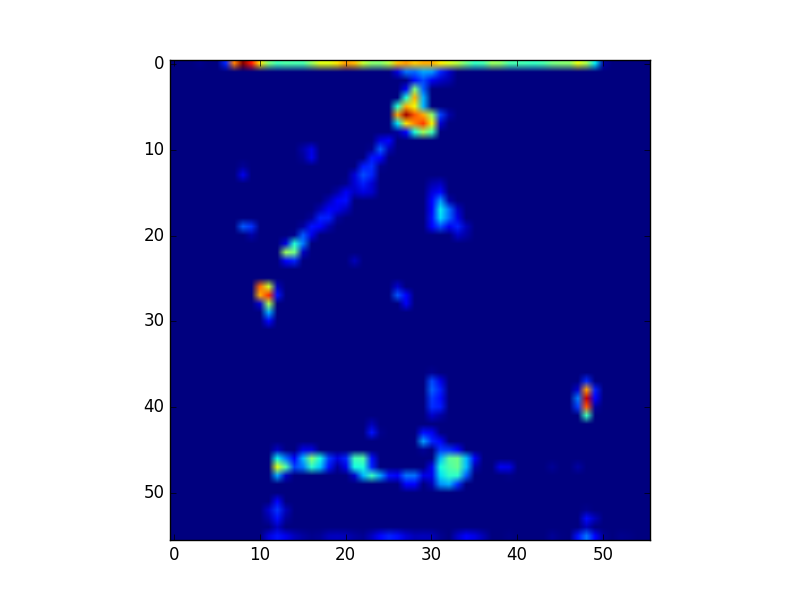
\includegraphics[width=\linewidth]{activation1.png}
\endminipage\hfill
\minipage{0.32\textwidth}
  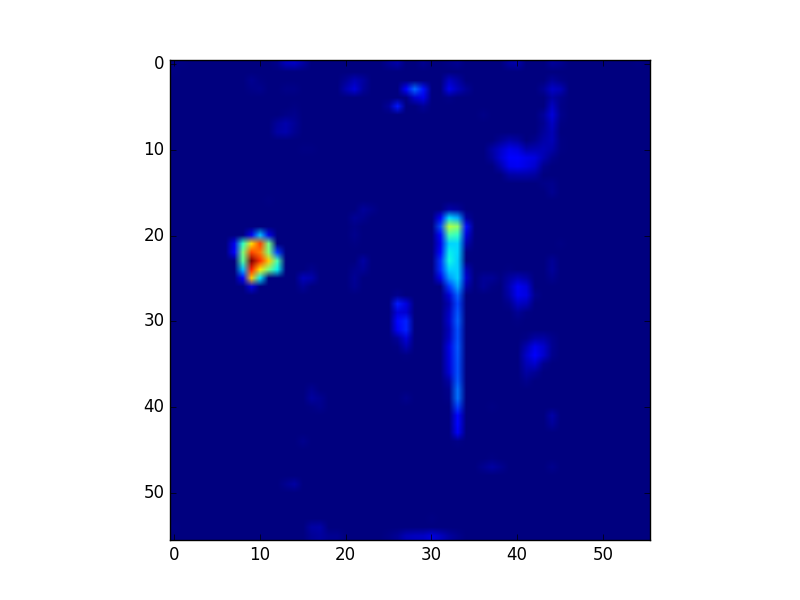
\includegraphics[width=\linewidth]{activation2.png}
\endminipage\hfill
\minipage{0.32\textwidth}%
  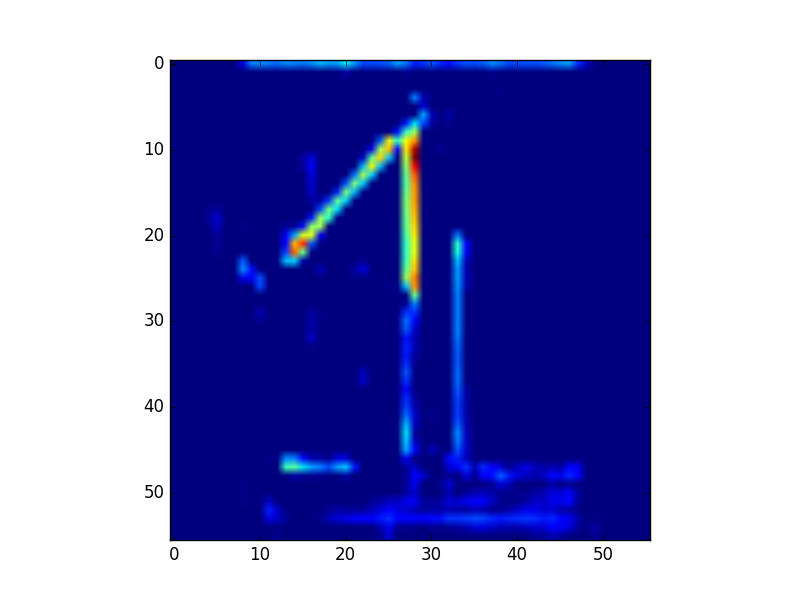
\includegraphics[width=\linewidth]{activation3.png}
\endminipage\hfill
  \caption{Activations at layer 15}
\end{figure}

\end{frame}

\begin{frame}
\frametitle{Pendulum position detection with activations}
\begin{itemize}
	\item Threshold on activations
	\item Clustering $\rightarrow$ center
	\item Video
\end{itemize}
\end{frame}


\begin{frame}
  \frametitle{Pendulum position}
  \begin{figure}
    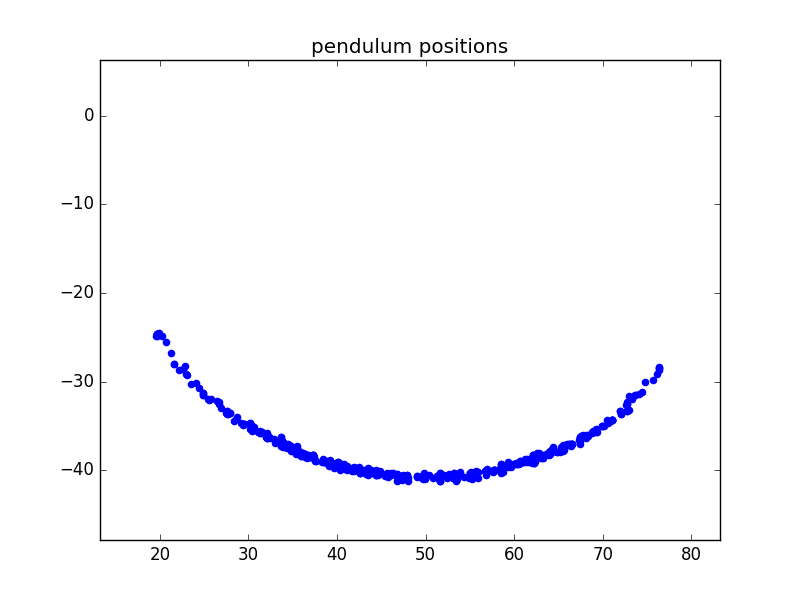
\includegraphics[height=7cm]{pendulum_positions.png}
  \end{figure}
\end{frame}

\begin{frame}
\frametitle{From pendulum position to pendulum angle}
To get the angles from the position we need to find the center $\rightarrow$ intesection of radius.
\begin{figure}
  \captionsetup{labelformat=empty}
  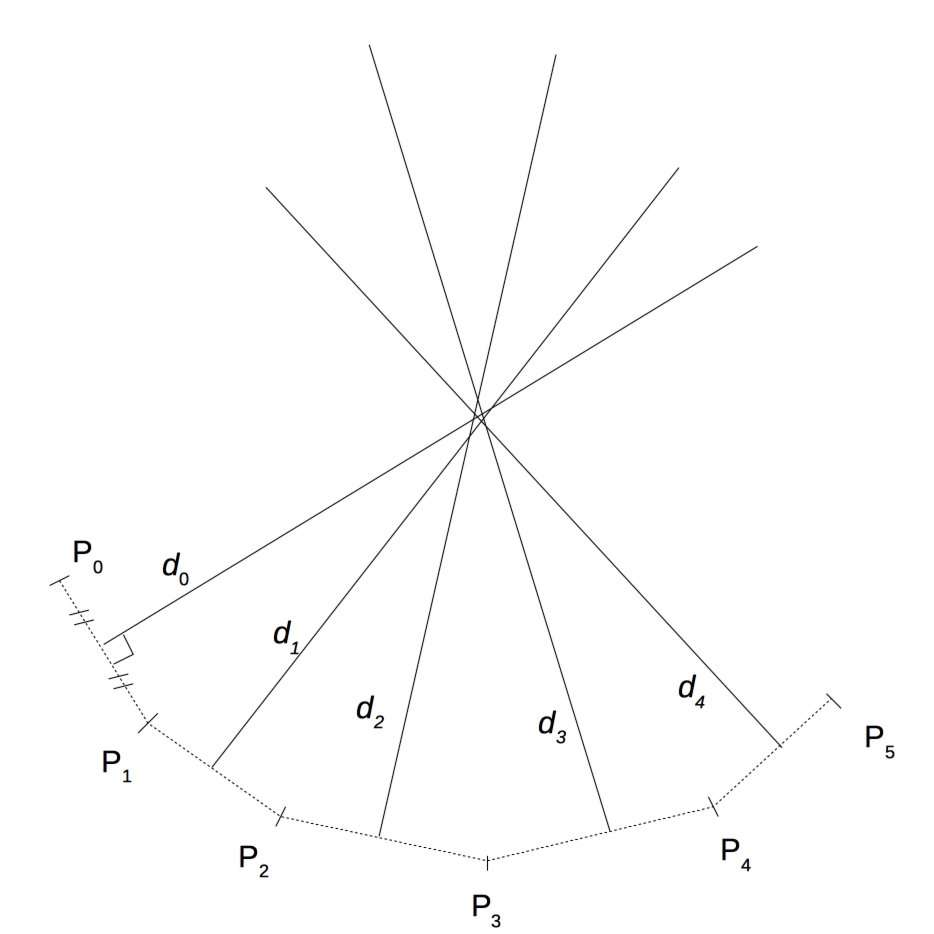
\includegraphics[height=3.5cm]{find_center.png}
  \caption{Find the intersection of lines $d_i$}
\end{figure}
The line will not exactly intersect $\rightarrow$ solve least square problem (gradient descent):
\[
  x = \text{argmin }\sum_i distance(x, d_i)^2
\]
\end{frame}

\begin{frame}
  \frametitle{Pendulum center}
  \begin{figure}
    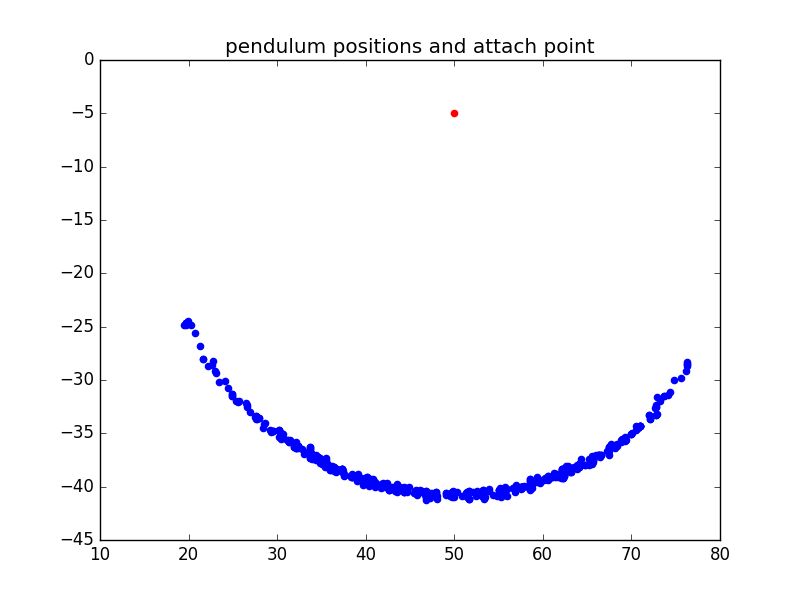
\includegraphics[height=7cm]{pendulum_positions_with_center.png}
  \end{figure}
\end{frame}

\begin{frame}
  \frametitle{Pendulum angles}
  \begin{figure}
    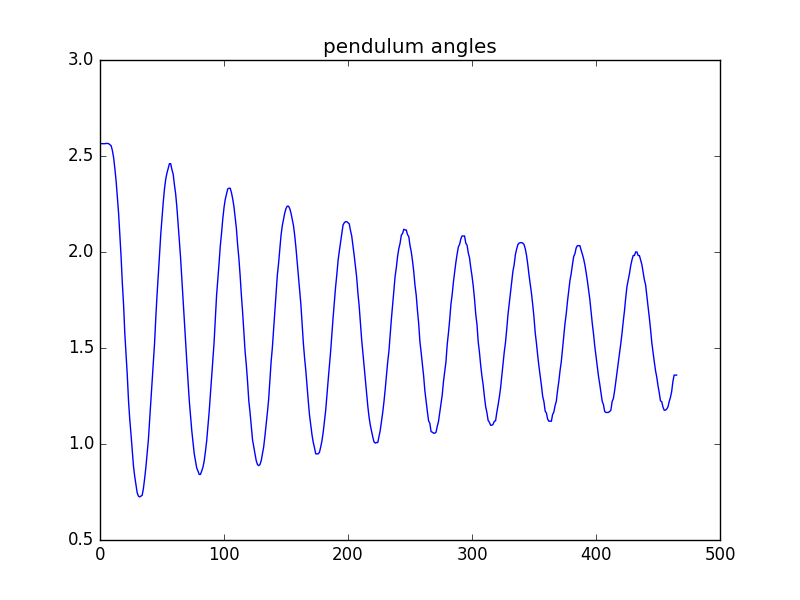
\includegraphics[height=4cm]{pendulum_angles.png}
  \end{figure}
  Estimation of the length with the period equal to $N / FPS = 50 / 31$.
  \begin{align*}
    T = \frac{N}{FPS} = 2 \pi \sqrt{\frac{l}{g}} &\implies l = g \left( \frac{N}{2 \pi FPS} \right)^2\\
    l  = 0.64m &\\
  \end{align*}
\end{frame}


\section{From angle sequence to pendulum length}

\begin{frame}
\frametitle{One step integration of pendulum equation}
With two successive angles $\theta_0$ and $\theta_1$, simple Euler integration :
\begin{align*}
  \left( \begin{array}{c} \theta_0 \\ \dot{\theta_0} \end{array} \right)&=
    \left( \begin{array}{c} \theta_0 \\ \frac{\theta_1 - \theta_0}{dt} \end{array} \right) \\
  \left( \begin{array}{c} \theta_1 \\ \dot{\theta_1} \end{array} \right) &=
    \left( \begin{array}{c} \theta_0  + dt \dot{\theta_0} \\ \dot{\theta_0} + dt \ddot{\theta_0} \end{array} \right)
    =
    \left( \begin{array}{c} \theta_1 \\ \dot{\theta_0} - dt \frac{g}{l} \sin(\theta_0) \end{array} \right)\\
  \left( \begin{array}{c} \theta_2 \\ \dot{\theta_2} \end{array} \right) &=
    \left( \begin{array}{c} \theta_1  + dt \dot{\theta_1} \\ \dot{\theta_1} + dt \ddot{\theta_1} \end{array} \right)
    =
    \left( \begin{array}{c} \theta_1 + dt \frac{\theta_1 - \theta_0}{dt} - dt^2 \frac{g}{l} \sin(\theta_0) \\ \ldots \end{array} \right)\\
\end{align*}
\[
  \theta_2 (l) = \theta_1 + dt \frac{\theta_1 - \theta_0}{dt} - dt^2 \frac{g}{l} \sin(\theta_0)
\]
\end{frame}

\begin{frame}
\frametitle{Deduce the length from three angles}
Assume we have three succesive angles $\theta_0$, $\theta_1$ and $\theta_2$.
Solve :
\begin{align*}
  \hat{l} &= \text{argmin } F(l)\\
  F(l) &= \left( \theta_2(l) - \theta_2 \right)^2\\
\end{align*}
Since $l \mapsto \theta_2(l)$ is stricly monotonous, F stricly convex $\rightarrow$ solve with gradient descent.
\begin{figure}
  \captionsetup{labelformat=empty}
  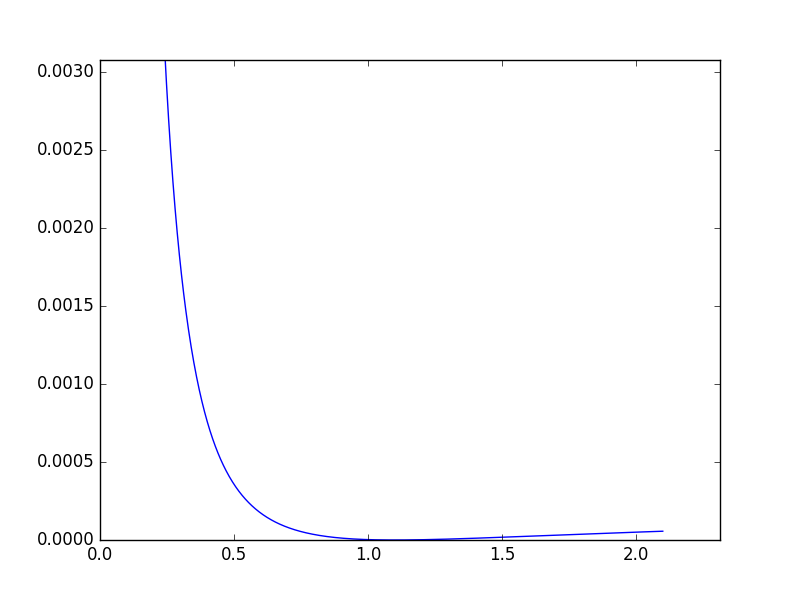
\includegraphics[height=3cm]{F.png}
  \caption{Function F}
\end{figure}
\end{frame}

\begin{frame}
\frametitle{Deduce the length}
$N$ angle observations $(\theta_0, \ldots, \theta_{N-1})$ noisy.
\begin{itemize}
  \item extract $N-2$ sequences of 3 angles :
    $\left( (\theta_0, \theta_1, \theta_2), (\theta_1, \theta_2, \theta_3), \ldots , (\theta_{N-3}, \theta_{N-2}, \theta_{N-1}) \right)$
  \item learn $N-2$ length correponding to these sequences
  \item average learned length
\end{itemize}
\end{frame}

\begin{frame}
\frametitle{Results}
  Result of the algorithm :
  \begin{align*}
    l  &= 0.62m \\
  \end{align*}
\end{frame}


\begin{frame}
\frametitle{Extensions}
\begin{itemize}
  \item Double pendulum:
    \begin{figure}
      \captionsetup{labelformat=empty}
      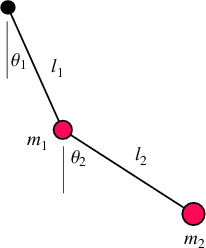
\includegraphics[height=4cm]{pendule_double.png}
      \caption{Double pendulum}
    \end{figure}
  \item Other techniques to find the pendulum position : KLT, ...
  \item Learning other parameters (friction coefficient)
  \item Other learning techniques (probabilistic...)
\end{itemize}
\end{frame}
\end{document}
